\documentclass[xcolor=dvipsnames,t]{beamer} % position stuff on top of slide
% Functions, packages, etc.
%[[[
\usetheme{Frankfurt}
\usecolortheme[named=Maroon]{structure}

% Remove Navigation Symbols
\usenavigationsymbolstemplate{}

\usepackage{amsmath}
\usepackage{amsfonts}
\usepackage{amssymb}
\usepackage{array}

\usepackage{tikz}

\usepackage{graphicx}
\usepackage{subfig}
\usepackage[labelfont=bf]{caption}
\captionsetup{font=small}
\usepackage{hyperref}

\newcommand{\tss}[1]{\textsuperscript{#1}}

\newcommand{\diff}[2]{\dfrac{d #1}{d #2}}
\newcommand{\diffn}[3]{\dfrac{d^{#3} #1}{d {#2}^{#3}}}
\newcommand{\pdiff}[2]{\dfrac{\partial #1}{\partial #2}}
\newcommand{\pdiffn}[3]{\dfrac{\partial^{#3} #1}{\partial {#2}^{#3}}}
\newcommand{\problemline}{\rule{\textwidth}{0.25mm}}
%\newcommand{\problem}[1]{\problemline\\#1\\\problemline\vspace{10pt}}
\newcommand{\reals}{\mathbb{R}}
\newcommand{\qline}[2]{\qbezier(#1)(#1)(#2)}
\newcommand{\abox}[1]{\begin{center}\fbox{#1}\end{center}}
%]]]

% Output Control Variables
\def\true{1}
\def\false{0}
\def\figures{1}
\def\tables{1}

\renewcommand{\UrlFont}{\scriptsize}
\newcommand{\defeq}{\mathrel{\mathop:}=}

% beamer description align left template
% http://tex.stackexchange.com/questions/95964/right-description-list-latex-beamer
\defbeamertemplate{description item}{align left}{\insertdescriptionitem\hfill}


\title{Automated Music Genre Classification}
\date{3 December, 2014}
\author{James Folberth, Aly Fox, Dale Jennings}

\begin{document}

\begin{frame}
\maketitle
\end{frame}

% TODO: these items are in no particular order and might not have the best names.  Please rename them and move them around as you wish.  Make sure that the section names match the names in the outline

\begin{frame}{Outline}
   %Outline:
   \setbeamertemplate{description item}[align left] % align left
   \begin{description}                              % align left
   %\setbeamertemplate{description item}[default]  % align right
   %\begin{description}[Clustering/Classification] % align right
      \item[Features] Spectral, Temporal, Wavelet Coefficient Histograms\\
      \item[Dimension Reduction] PCA, LLE, PageRank, Graph Laplacian\\
      \item[Clustering/Classification] kNN, SVM with multi-class, Graph Laplacian\\
      \item[Discussion]
   \end{description}

\end{frame}

\section{Features}
% Dale
\begin{frame}{Simple Features}
Time based features extracted from the raw wav vector.  For each feature, the mean, variance, skewness, and kurtosis is calculated.
\begin{itemize}
\item Autocorrelation Coefficient 20
\item Autocorrelation Maximum
\item Peak Envelope
\item Predictivity Ratio
\item Root Mean Square
\item Standard Deviation
\item Zero Crossing Rate
\end{itemize}
\end{frame}

% Dale
\begin{frame}{Spectral Features}
Extracted from the power spectrum of the song.  For each feature, the mean, variance, skewness, and kurtosis is calculated.
\begin{columns}[t]
\column{.5\textwidth}
\begin{itemize}
\item Spectral Centroid
\item Spectral Crest
\item Spectral Decrease
\item Spectral Flatness
\item Spectral Flux
\item Spectral Kurtosis
\item Spectral Rolloff
\end{itemize}
\column{.5\textwidth}
\begin{itemize}
\item Spectral Skewness
\item Spectral Slope
\item Spectral Spread
\item Tonal Power Ratio
\item Mel Frequency Cepstrum Coefficients (1-13)
\item Pitch Chroma (12 notes)
\end{itemize}
\end{columns}

% Dale
\end{frame}
\begin{frame}{Fluctuation Patterns}
Extracted from the Mel Frequency Cepstrum.
\begin{itemize}
\item Maximum Fluctuation Strength
\item Bass
\item Aggressiveness
\item Domination of Low Frequencies
\item Gravity
\item Focus
\end{itemize}

\end{frame}

% James
\begin{frame}{Wavelet Coefficient Histograms}
   \begin{columns}[T,onlytextwidth]
      \begin{column}{0.45\textwidth}
         \begin{itemize}
            \item The wavelet transform generally has good time and frequency resolution.
            \item Complex temporal signals become more simple in the wavelet domain.
            \item We look at the histogram of wavelet coefficients in each sub-band.
         \end{itemize}

      \end{column}

      \begin{column}{0.45\textwidth}
         The multiresolution idea:\\[1em]
         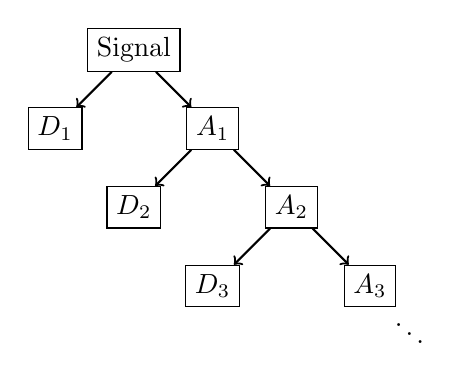
\begin{tikzpicture}
            \node[draw] (signal) at (0,0) {Signal};
            \node[draw] (a1) at (1,-1) {$A_1$};
            \node[draw] (d1) at (-1,-1) {$D_1$};

            \node[draw] (a2) at (2,-2) {$A_2$};
            \node[draw] (d2) at (0,-2) {$D_2$};

            \node[draw] (a3) at (3,-3) {$A_3$};
            \node[draw] (d3) at (1,-3) {$D_3$};

            \node (etc) at (3.5,-3.5) {$\ddots$};

            \draw[thick,->] (signal) -- (a1);
            \draw[thick,->] (signal) -- (d1);
            \draw[thick,->] (a1) -- (a2);
            \draw[thick,->] (a1) -- (d2);
            \draw[thick,->] (a2) -- (a3);
            \draw[thick,->] (a2) -- (d3);

         \end{tikzpicture}
      \end{column}
   \end{columns}
\end{frame}

% James
\begin{frame}{Wavelet Coefficient Histograms}
   Idea: The WCHs are characterized by their moments.\\

   ~\\
   The WCH features are extracted as follows:
   \begin{enumerate}
      \item Compute the wavelet decomposition of a central segment of the signal.
      \item Construct the histogram for each sub-band.
      \item Compute the first three moments of each histogram (mean, variance, skewness).
      \item Compute a sub-band energy for each histogram.
   \end{enumerate}

   % Not all subbands contain useful information
\end{frame}

% James
\begin{frame}{Wavelet Coefficient Histograms}
   Features from detail sub-bands $4,5,6,7$:\\

   ~\\[-10em]
   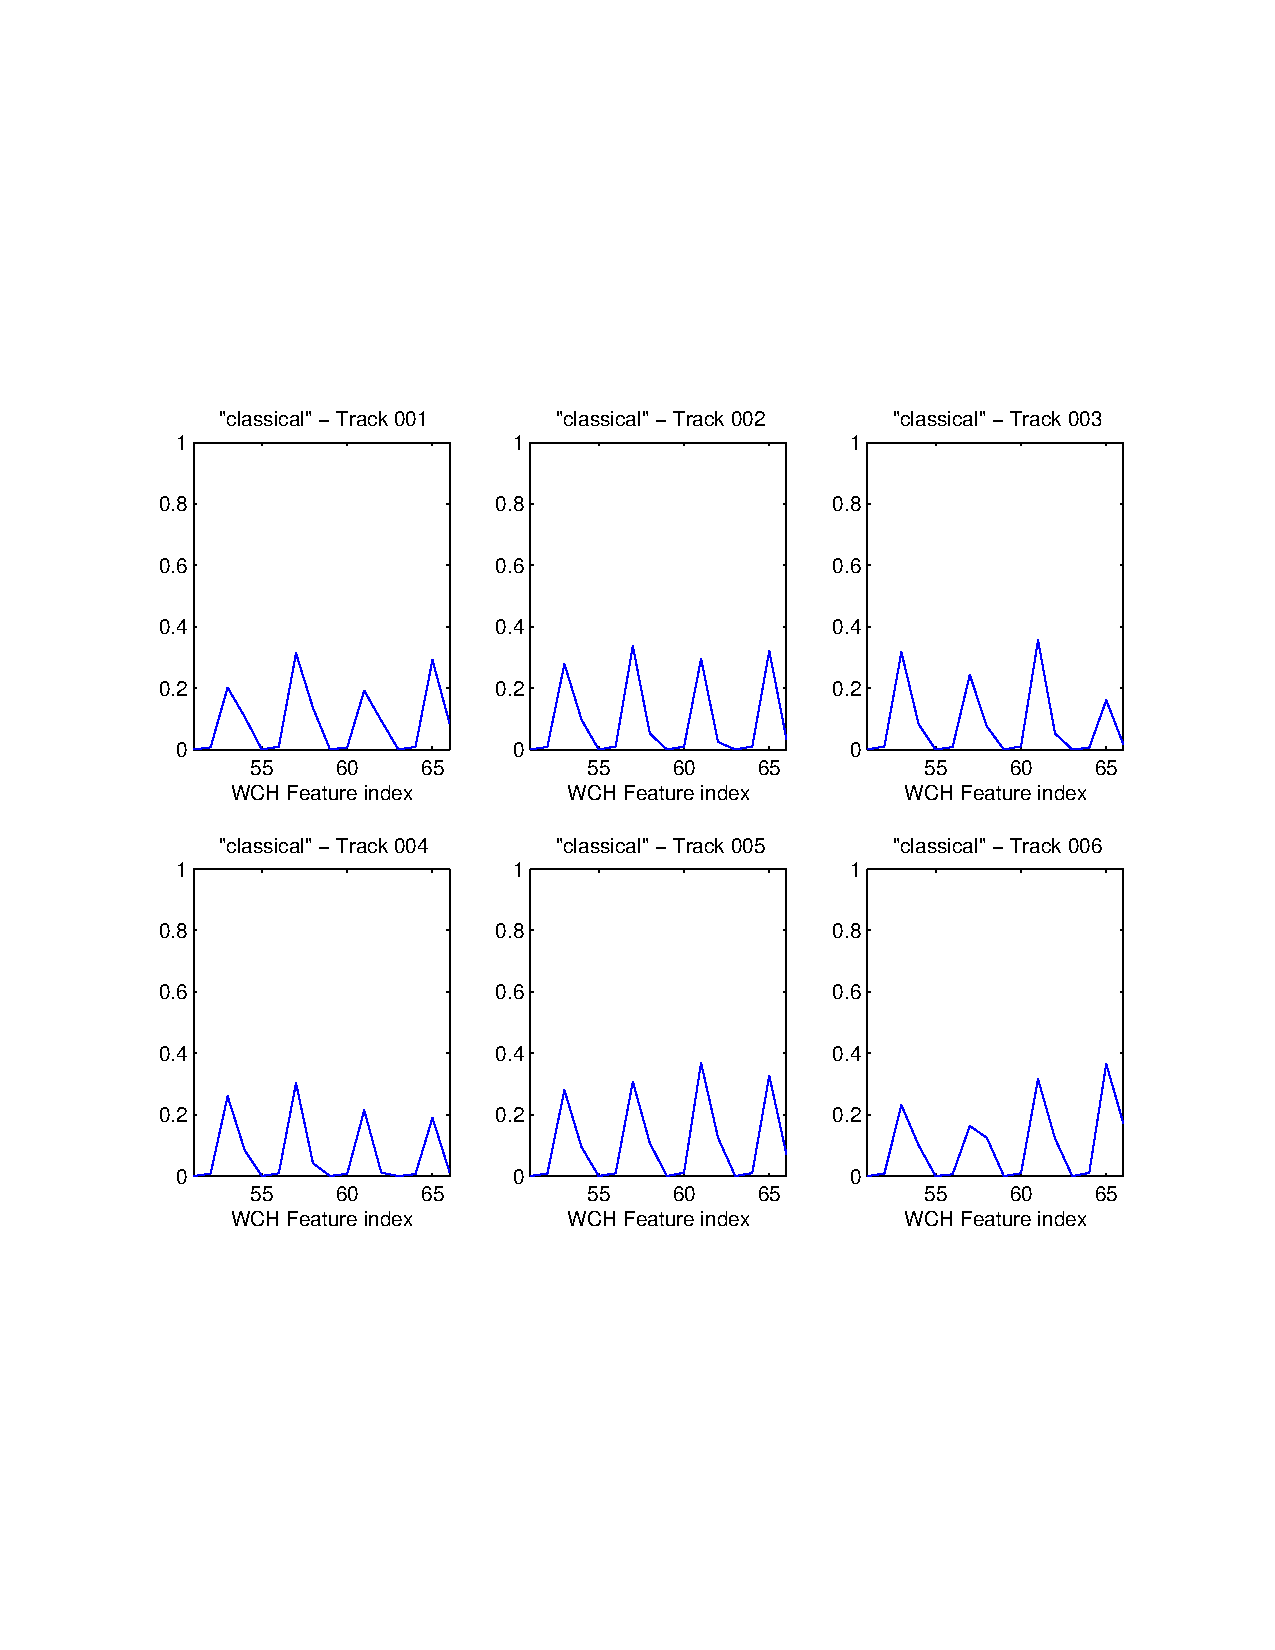
\includegraphics[width=\textwidth]{figures/wch_class.pdf}

\end{frame}

% James
\begin{frame}{Wavelet Coefficient Histograms}
   Features from detail sub-bands $4,5,6,7$:\\

   ~\\[-10em]
   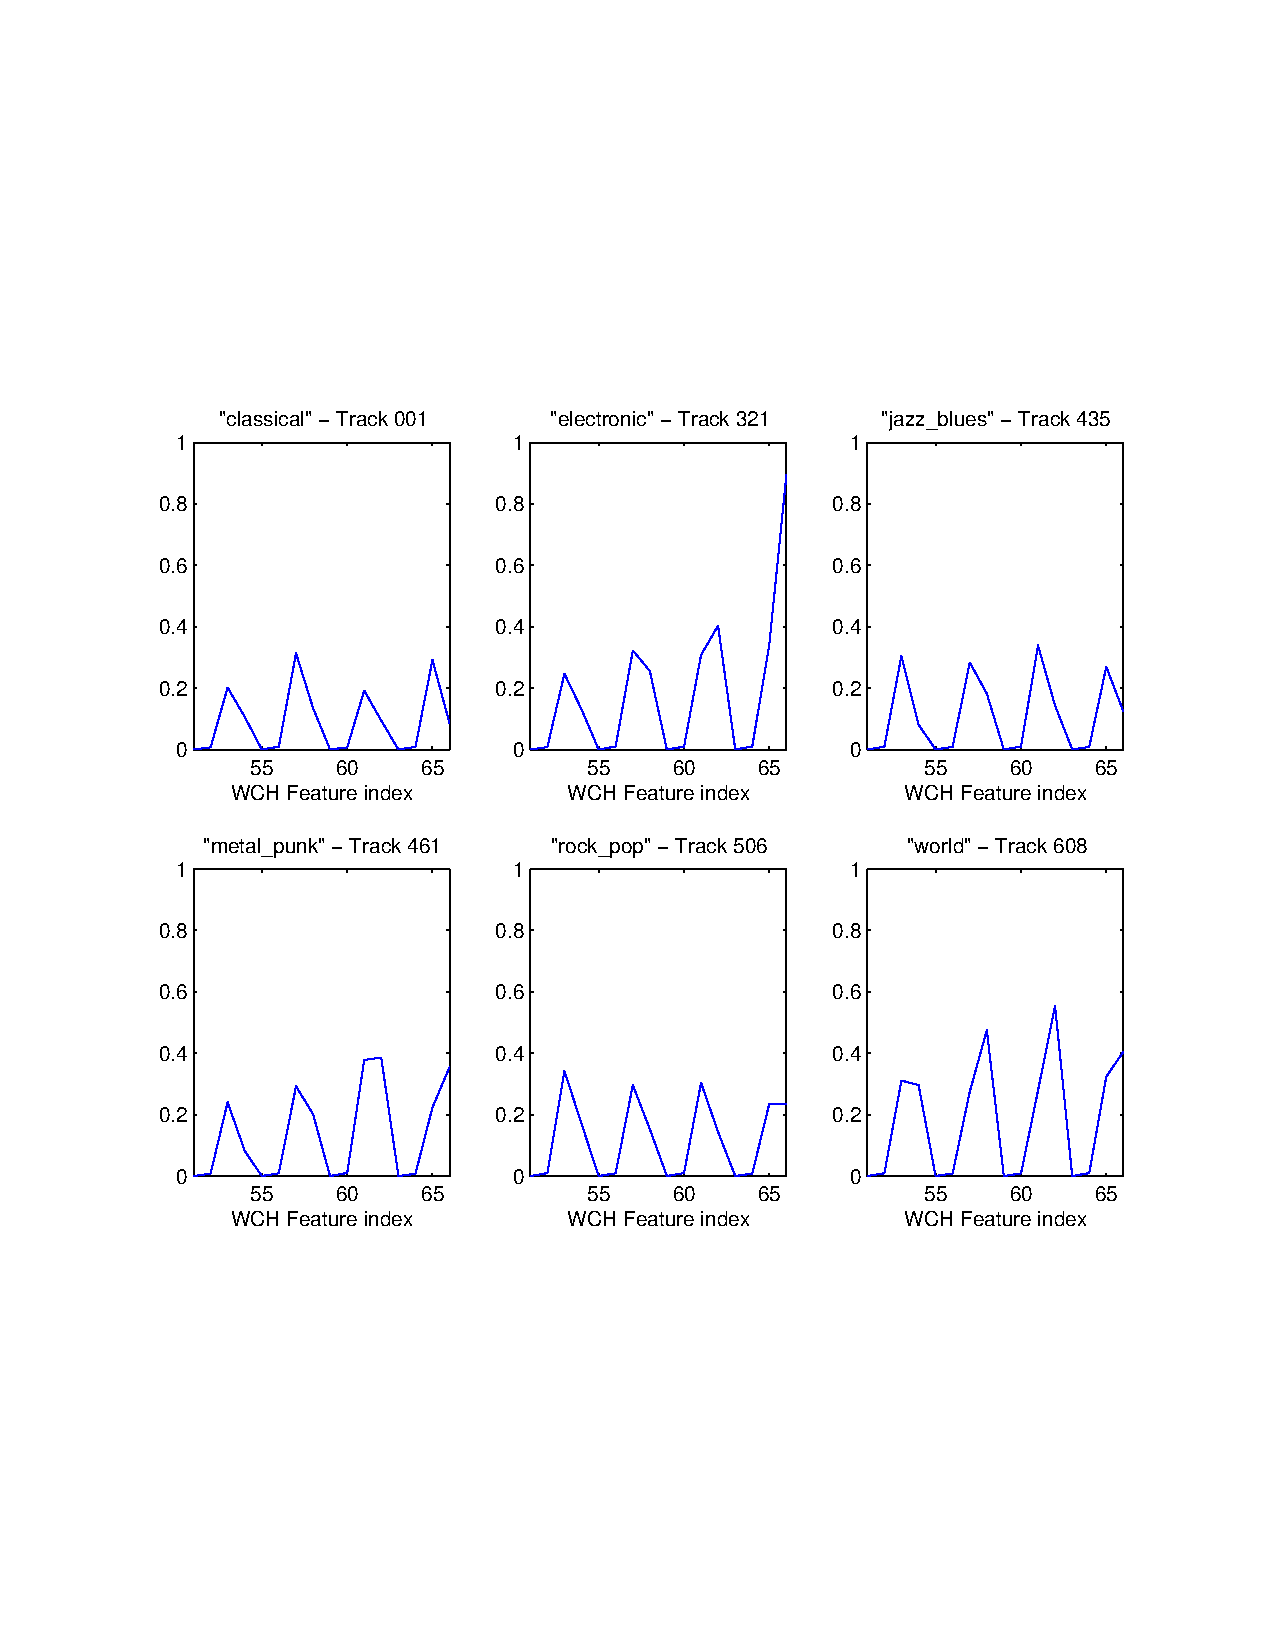
\includegraphics[width=\textwidth]{figures/wch_diff.pdf}

\end{frame}

% James
% Stolen from Li et al. SIGIR 2003
%\begin{frame}{Wavelet Coefficient Histograms}
%   \begin{columns}[T,onlytextwidth]
%      \begin{column}{0.25\textwidth}
%         From Li et al., \emph{SIGIR} '03.\\
%      \end{column}
%
%      \begin{column}{0.7\textwidth}
%         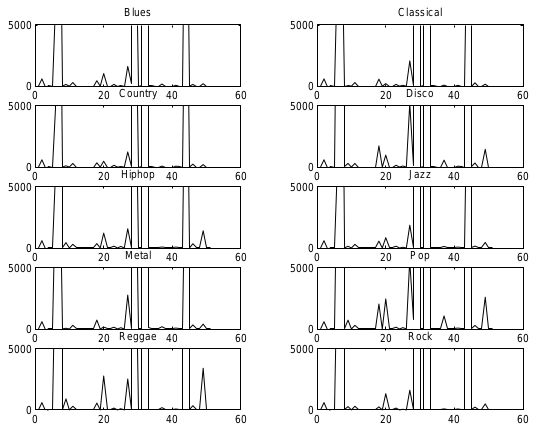
\includegraphics[width=\textwidth]{figures/wch_li_1.png}
%      \end{column}
%   \end{columns}
%\end{frame}

\begin{frame}{Combining Features into Distances}

\begin{itemize}
\item Once we have computed various features and similarity measures we can combine them into a "distance" in a meaningful way. 
\item One option is to use a convex combination of the $z$ (standard) scores of the distances. This method gives the combined distance:
 \[ d = \sum_{i} w_i \left(\dfrac{d_i - \mu_i}{\sigma_i}\right) + \text{offset}, \]
 where  $w_i\ge 0$, $\sum_i w_i=1$, $d_i$ is the $i$th distance (with a specific feature) to be combined and $\mu_i$ and $\sigma_i$ are the mean and standard deviation of the $i$th distance to be able to standardize. 
 \end{itemize}
 \end{frame}
 \begin{frame}{Combining Features into Distances}

\begin{itemize}
 \item We compute this over over some reference set of songs and the offset is chosen so that the distance is positive for each pair of songs.
 \item This creates a "Distance" matrix of all the reference songs. 
  \item We use a single Gaussian to cluster the MFCC frames for each track, and then compare the cluster models between two tracks using the rescaled KL- divergence. We also compute the median fluctuation patterns, bass, and center of gravity. 
 \item Pampalk describes a few possible combinations, we chose use the combination called G1C. It combines the features using the weights 0.7 for the spectral similarity, and 0.1 each for median fluctuation pattern, bass, and center of gravity.
 \end{itemize}
\end{frame}

\begin{frame}[shrink=20]{Base Method for Classifying}
Using K-nearest neighbors with $k=5$ and leave-out-$p$-cross-validation we have the following results:
\begin{table}[h!]
\centering
%\input{../crossValAvg.tex}
 \begin{tabular}{ l||l | l | l | l | l | l | }
 & classical & electronic & jazz\_blues & metal\_punk & rock\_pop & world\\\hline
classical & 63 &1 &2 &0 &1 &10 \\ \hline 
electronic & 0 &16 &0 &0 &1 &3 \\ \hline 
jazz\_blues & 0 &0 &1 &0 &0 &0 \\ \hline 
metal\_punk & 0 &0 &0 &4 &3 &0 \\ \hline 
rock\_pop & 0 &5 &2 &4 &16 &7 \\ \hline 
world & 1 &1 &0 &0 &0 &5 \\ \hline 
\end{tabular}

\caption{(Rounded) Average of the Confusion Matrices}
\label{fig:avgconfMat}
\end{table}
\end{frame}

\begin{frame}[shrink=20]{Base Method for Classifying}
\begin{table}[h!]
\centering
%\input{../crossValSD.tex}
 \begin{tabular}{ l||l | l | l | l | l | l | }
 & classical & electronic & jazz\_blues & metal\_punk & rock\_pop & world\\\hline
classical & 0.77 &0.65 &1.22 &0.40 &0.86 &1.96 \\ \hline 
electronic & 0.00 &1.97 &0.27 &0.40 &0.80 &1.70 \\ \hline 
jazz\_blues & 0.00 &0.00 &0.96 &0.00 &0.00 &0.33 \\ \hline 
metal\_punk & 0.00 &0.47 &0.00 &1.40 &1.67 &0.36 \\ \hline 
rock\_pop & 0.30 &1.65 &1.14 &1.42 &1.93 &1.83 \\ \hline 
world & 0.78 &0.88 &0.59 &0.00 &0.35 &1.84 \\ \hline 
\end{tabular}

\caption{Standard Deviation of the Confusion Matrices}
\label{fig:stdconfMat}
\end{table}
The percent correct for each genre are as follows,
   \[ [98.44\%, 69.57\%,20.00\%,50.00\%,76.19\%,20.00\%]. \]
 with the probability correct is $55.7\%$.
\end{frame}


\section{Dimension Reduction}
% James
\begin{frame}{Principal Component Analysis}
   Some literature suggests that PCA \emph{may} work, but one should be careful.  Clustering with PCs may not work well.

   ~\\[-7em]
   \begin{figure}
      \centering
      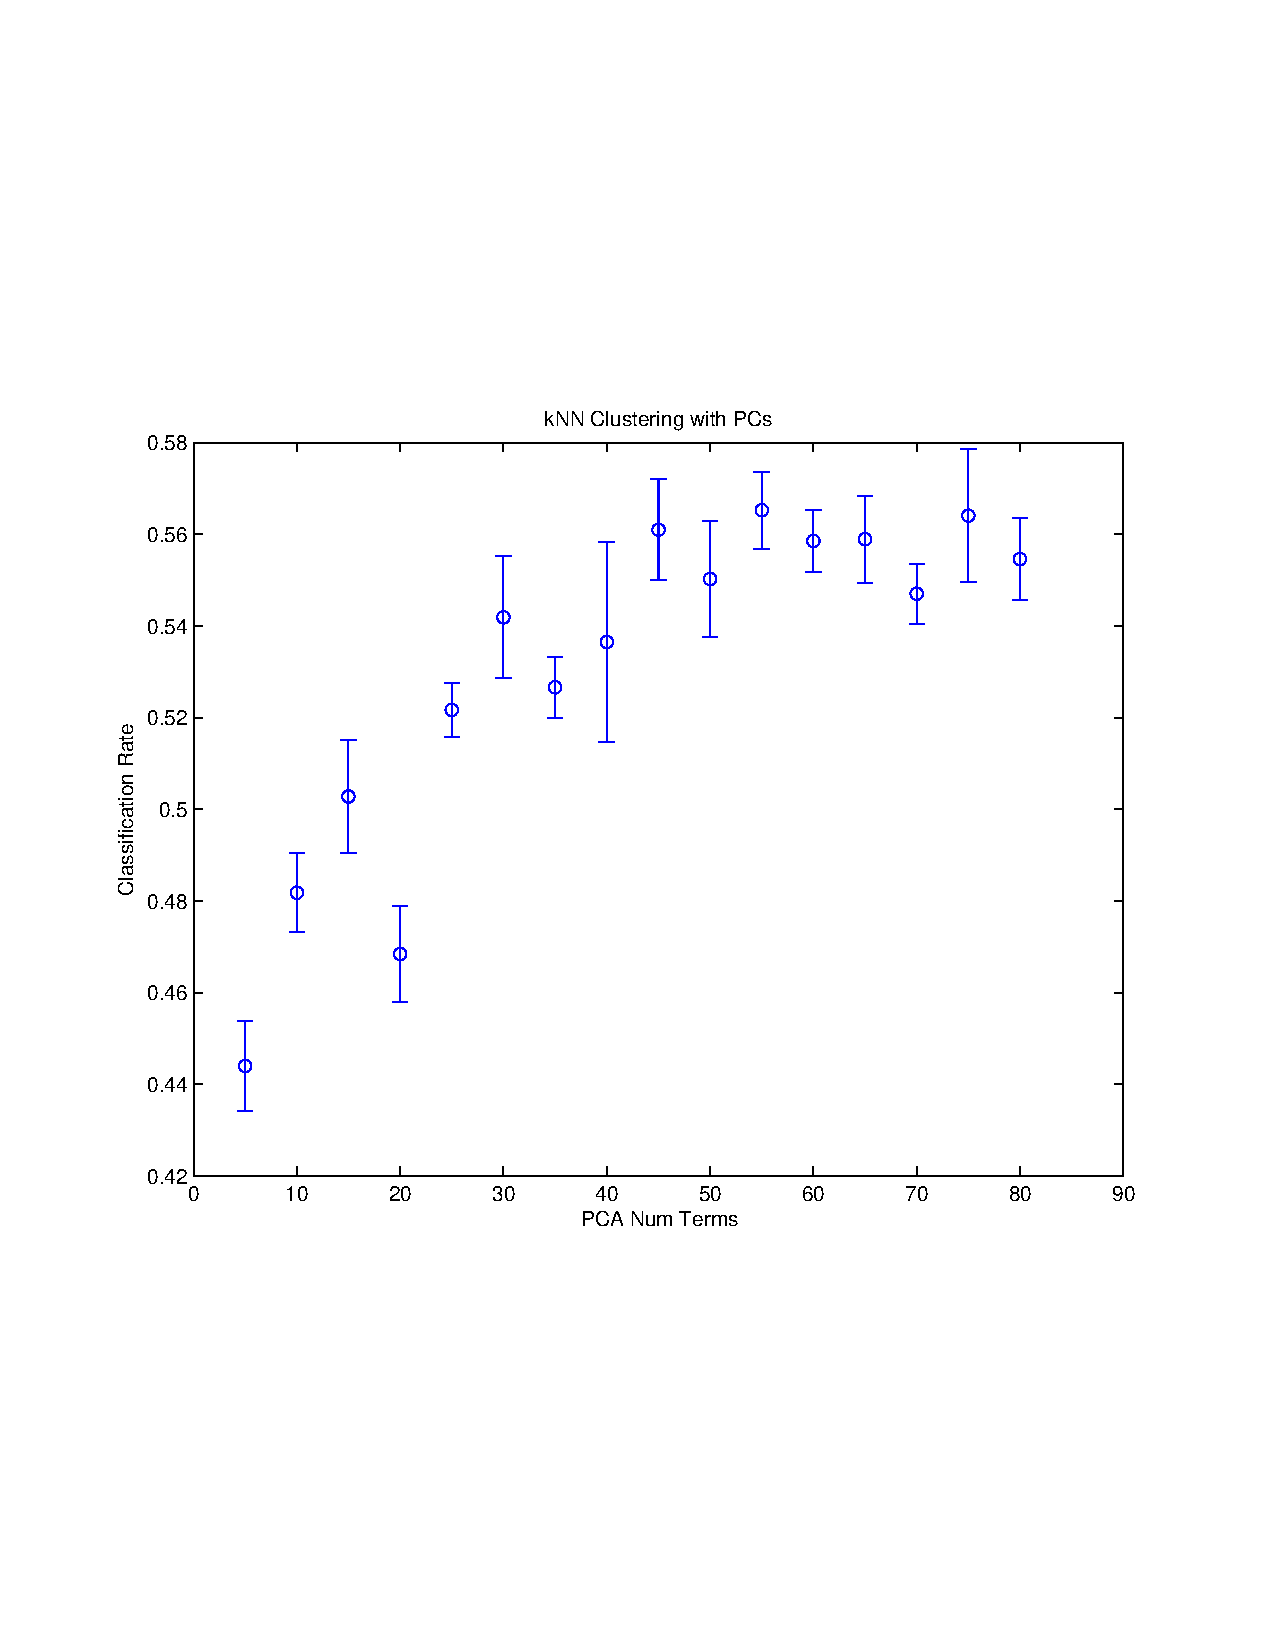
\includegraphics[width=0.8\textwidth]{figures/optimkNNPCA.pdf}
   \end{figure}
\end{frame}

% James
\begin{frame}{Locally Linear Embedding}
   We also tried LLE.  It doesn't work quite as well as PCA.

   ~\\[-7em]
   \begin{figure}
      \centering
      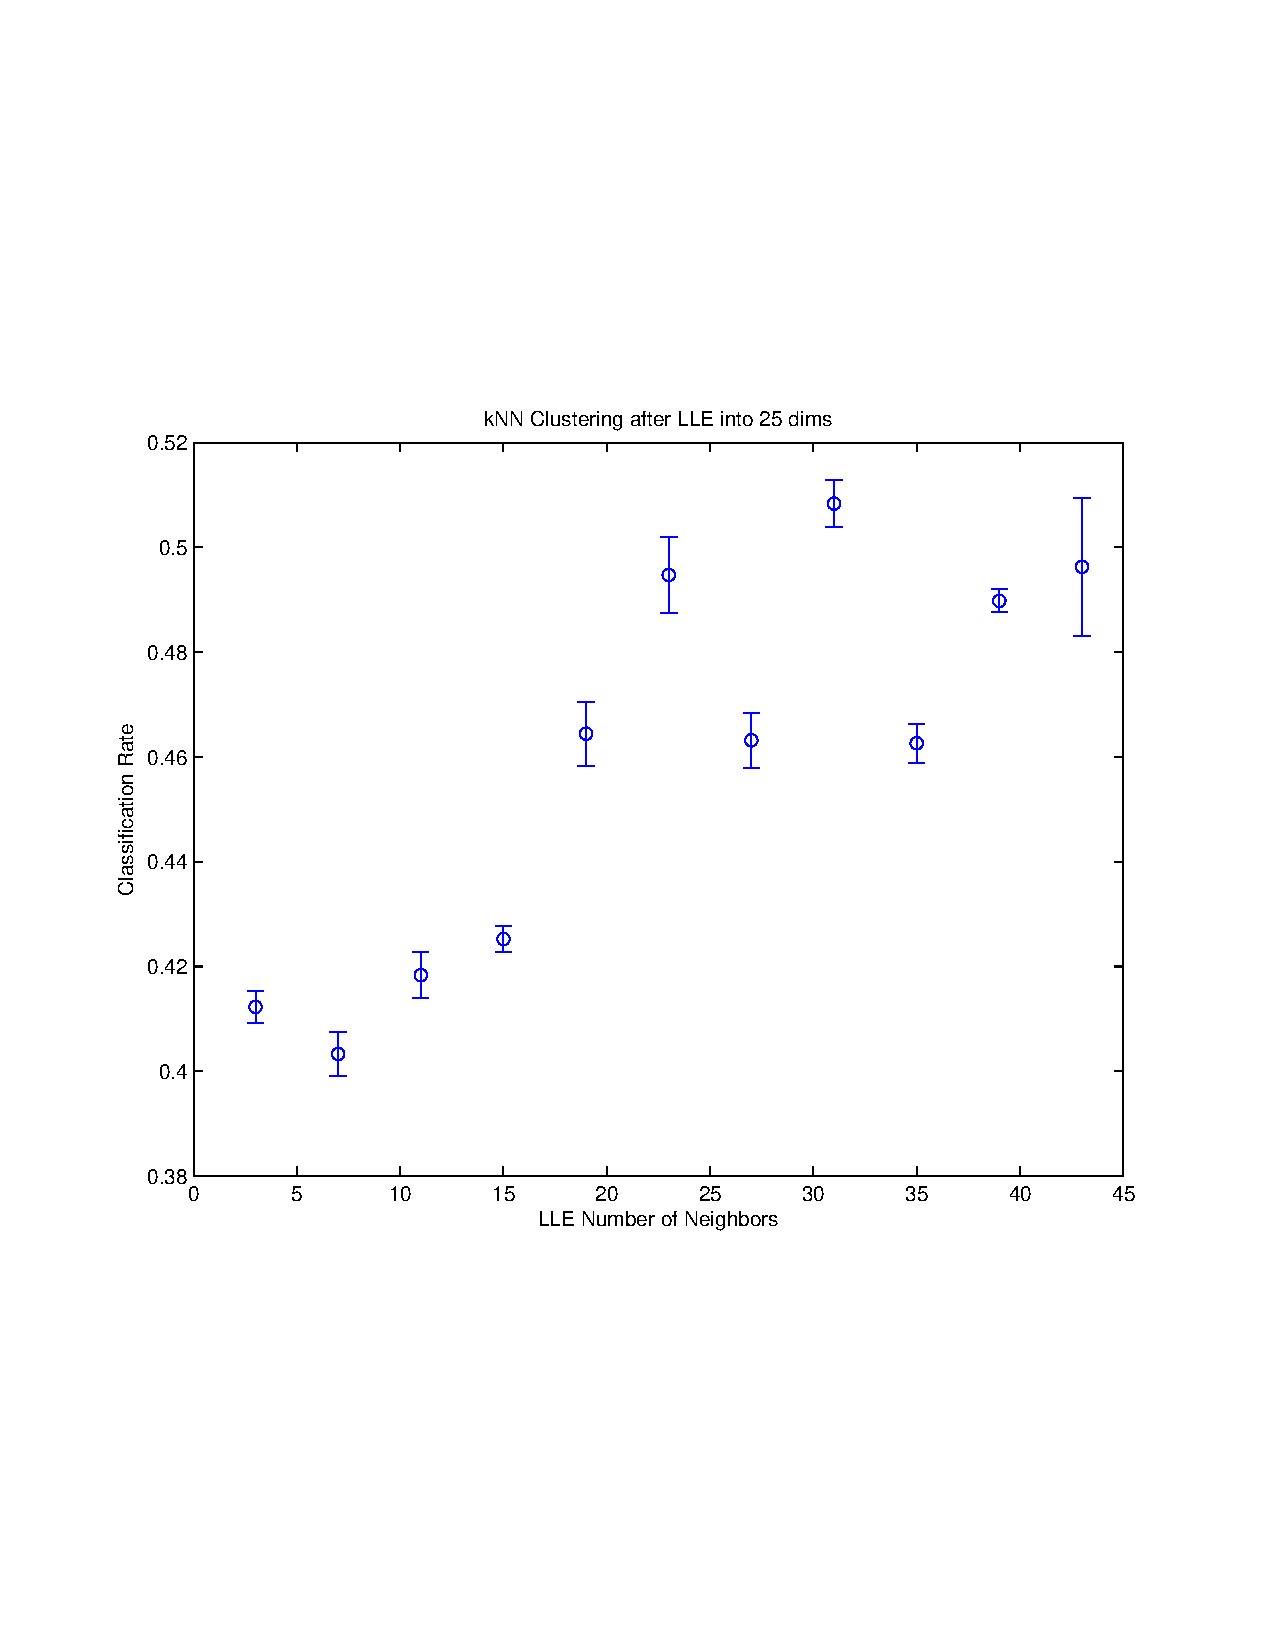
\includegraphics[width=0.8\textwidth]{figures/optimkNNLLE.pdf}
   \end{figure}
\end{frame}

% Dale
\begin{frame}{PageRank feature selection}
\begin{itemize}
\item Most dimension reduction techniques require a projection from higher dimensional space
\item In the music context, this means extracting all originally considered features
\item No reduction in feature extraction cost
\item Ideally, want to choose a subset of all possible features that can be used to accurately classify the data
\end{itemize}
\end{frame}

\begin{frame}{PageRank feature selection}
\textbf{Idea:} Construct a graph with nodes as features.  Edge weights are squared Spearman correlations between the features. Run the page rank algorithm to find the ``best'' features.

\begin{figure}
\centering
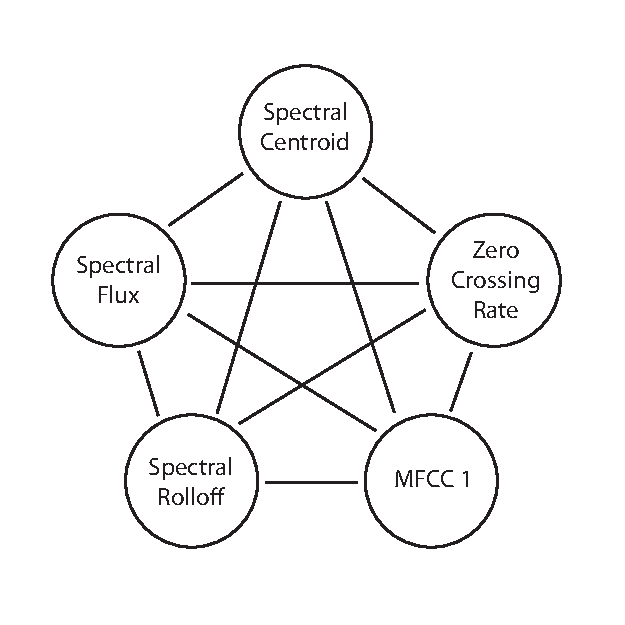
\includegraphics[width=0.4\textwidth]{figures/featGraph.pdf}
\end{figure}
\end{frame}

\begin{frame}{PageRank feature selection}
\begin{itemize}
\item Correlation creates a dense graph, no need for arbitrary escape probabilities
\item Damping can still be included, but wasn't for these experiments
\item In a naive approach, all songs are considered when calculating the correlations
\end{itemize}

\begin{center}
\begin{tabular}{|l|l|}
\hline
Rank & Feature \\ \hline
1 & Mfcc 1\tss{(1)} \\ \hline
2 & Spectral Flatness\tss{(1)} \\ \hline
3 & Peak Envelope Max\tss{(1)} \\ \hline
4 & Spectral Slope\tss{(1)} \\ \hline
5 & Autocorrelation Max\tss{(1)} \\ \hline
\end{tabular}
\end{center}

\end{frame}

\begin{frame}{PageRank feature selection}
\begin{itemize}
\item Considering all songs together assumes that the best features are independent of genre
\item In a more sophisticated approach, the features are ranked for each genre individually
\end{itemize}

\begin{columns}[t]
\column{.5\textwidth}
\begin{center}
\textbf{Classical:}
\begin{tabular}{|l|l|}
\hline
Rank & Feature \\ \hline
1 & Zero Crossing Rate\tss{(1)} \\ \hline
2 & Spectral Centroid\tss{(1)} \\ \hline
3 & Spectral Spread\tss{(1)} \\ \hline
4 & Spectral Rolloff\tss{(1)} \\ \hline
5 & Spectral Crest\tss{(1)} \\ \hline
\end{tabular}
\end{center}
\column{.5\textwidth}
\begin{center}
\textbf{Jazz/Blues:}
\begin{tabular}{|l|l|}
\hline
Rank & Feature \\ \hline
1 & Spectral Rolloff\tss{(2)} \\ \hline
2 & Mfcc 3\tss{(2)} \\ \hline
3 & FP DLF \\ \hline
4 & Mfcc 5\tss{(1)} \\ \hline
5 & FP Bass \\ \hline
\end{tabular}
\end{center}
\end{columns}
\end{frame}

\begin{frame}{PageRank feature selection}
\textbf{Combined Method:}
\vspace{-1in}
\begin{figure}
\centering
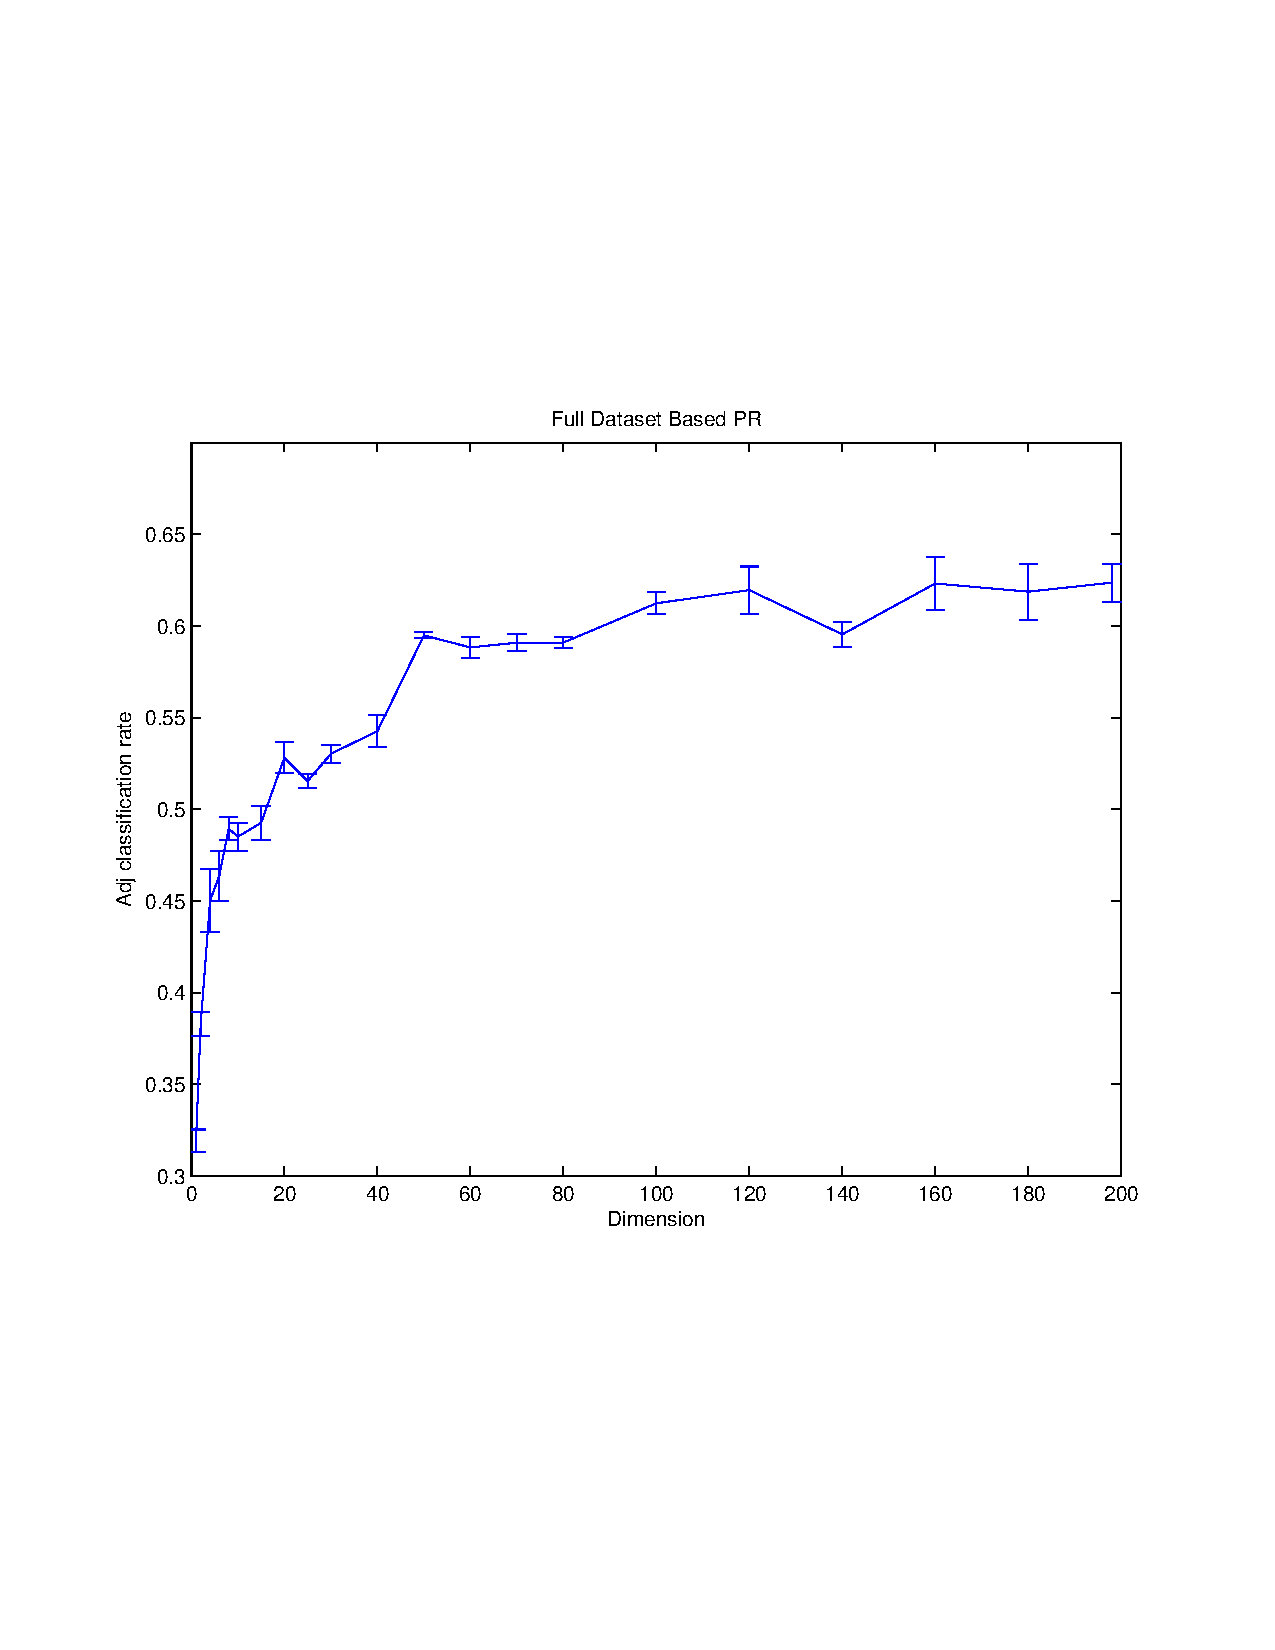
\includegraphics[width=0.9\textwidth]{figures/fullPR.pdf}
\end{figure}

\end{frame}

\begin{frame}{PageRank feature selection}

\textbf{Genre Divided Method:}
\vspace{-1in}
\begin{figure}
\centering
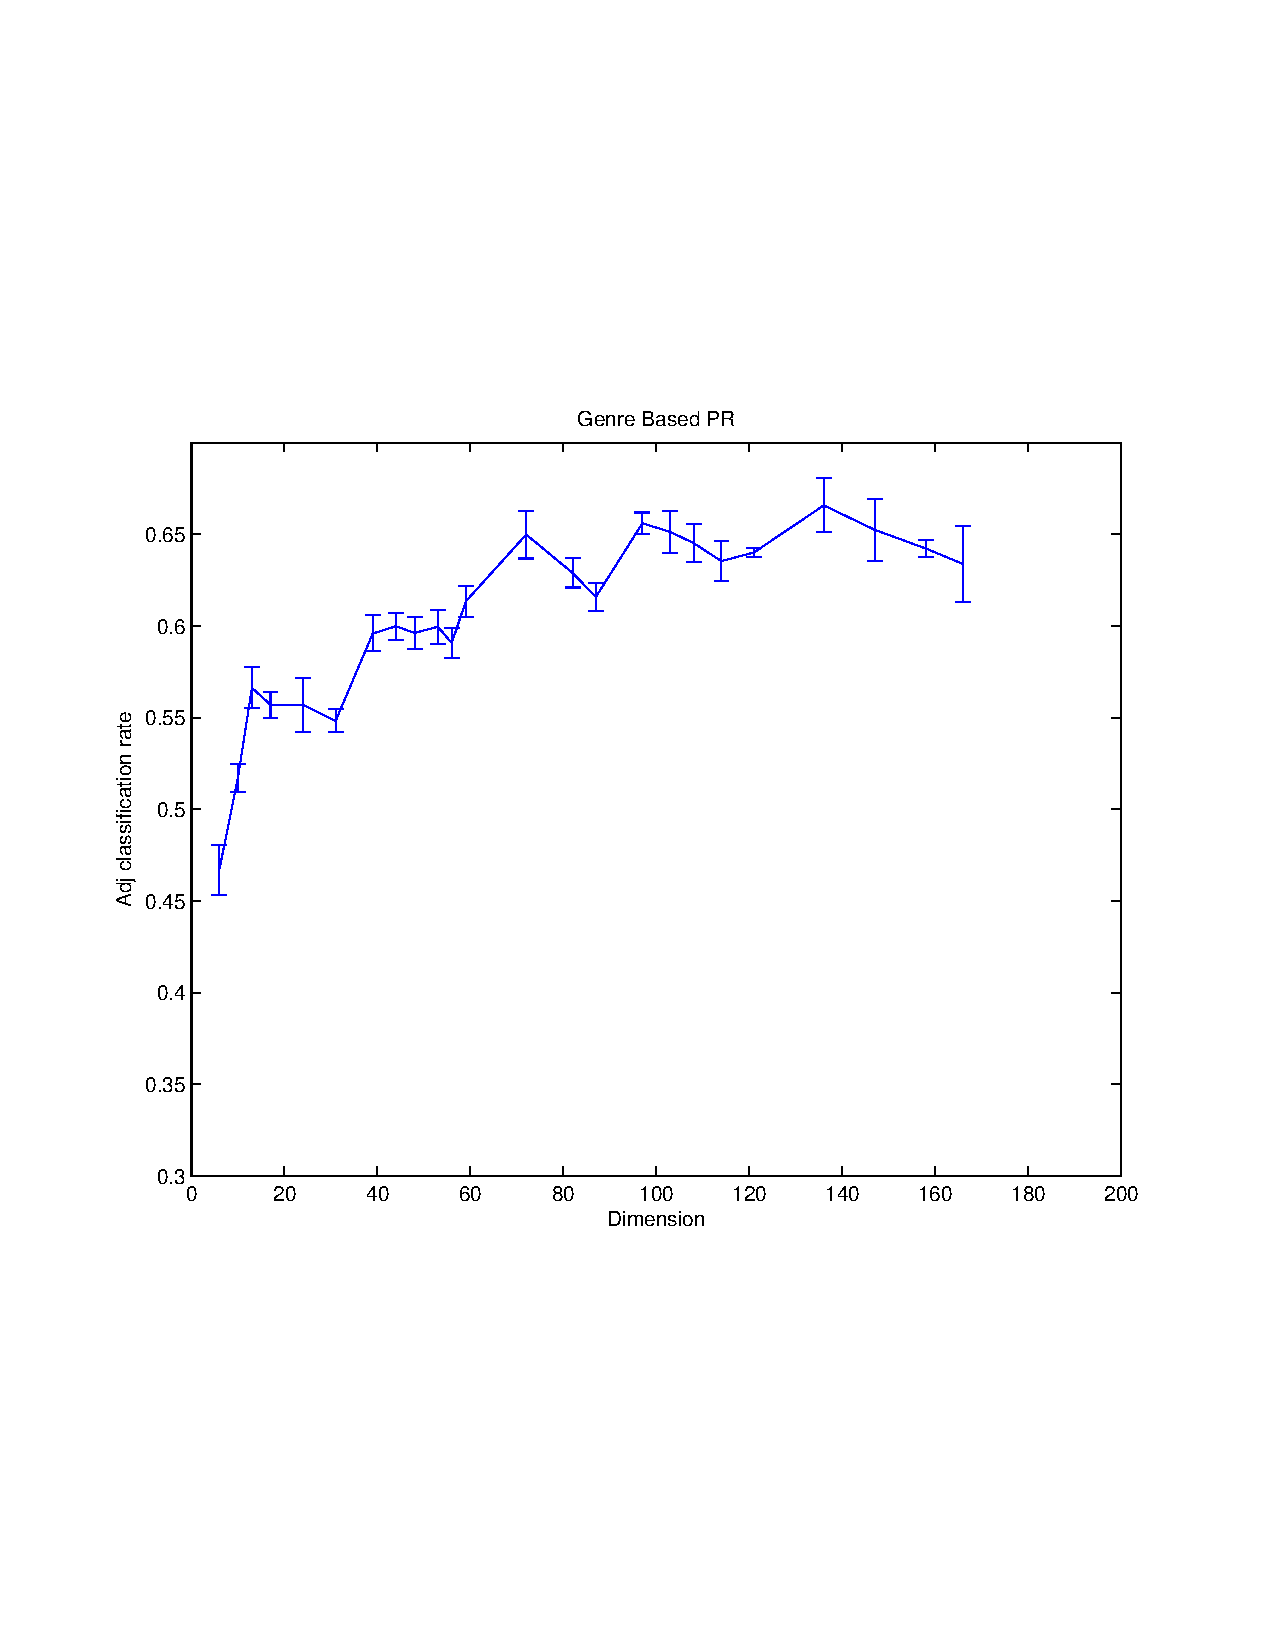
\includegraphics[width=0.9\textwidth]{figures/genrePR.pdf}
\end{figure}

\end{frame}

% Dale
%\begin{frame}{Manually selecting features}
%   \begin{itemize}
%      \item A na\"ive option is to manually select some number of features from a large list of features.  We use this mainly for testing.
%      \item We combined various simple features, the mean and variance of the MFCCs, and features from the WCHs into a length $66$ vector.
%      \item We'll show how this performs when we discuss SVM.
%   \end{itemize}
%\end{frame}

\begin{frame}{Graph Representations}
\begin{itemize}
\item If we only have some similarity between data points we can represent the data in a similarity graph $G = (V,E)$ where $V$ is the set of vertices and $E$ is the weighted edges. 
\item From the distance matrix, extracted from the features, we can build a similarity graph between the set of songs. 
\item This results is a sparse representation of the data.
\item Before we create the graph, we normalized the distance matrix so that  each entry is between zero and one. 
\item There are three methods to attain the similarity {\bf{adjacency}} matrix:
\begin{itemize}
\item  $\epsilon$-neighborhood graph = chose only distances that are less than a certain $\epsilon$ and and zeros the other entries. 
\item $k$-nearest neighbor graph = find $k$ nearest neighbors and only keep those distances.
\item Fully connected graph= keep all distances. 
\end{itemize}
\end{itemize}
\end{frame}

\begin{frame}{Spectral Clustering with Graph Laplacians}
Spectral clustering is a method of using the spectrum of a matrix in order to preform dimensionality reduction before clustering. This allows us to cluster in fewer dimensions. We have three main  methods in which to compute the Spectral Clustering:
\begin{itemize}
\item Unnormalized:
\begin{enumerate}
\item Computed the unnormalized graph Laplacian, $L$,from the similarity adjacency matrix.  
\item Compute the associated eigenvectors of the first (magnitude) $k$ eigenvalues of $L$ and store them in the matrix $V$. 
\item Using the rows of $V$  as our spectral coordinates for clustering the points. 
\end{enumerate}
\end{itemize}
\end{frame}

\begin{frame}{Spectral Clustering with Graph Laplacians}
\begin{itemize}
\item Normalized Method 1:
\begin{enumerate}
\item Computed the unnormalized graph Laplacian $L$ from the similarity adjacency matrix.  
\item Compute the associated eigenvectors of the first (magnitude) $k$ eigenvalues of the system, $Lv = \lambda Dv$ and store them in the matrix $V$. 
\item Using the rows of $V$  as our spectral coordinates for clustering the points. 
\end{enumerate}

\item Normalized Method 2:
\begin{enumerate}
\item Computed the normalized graph Laplacian $L$ from the similarity adjacency matrix.  
\item Compute the associated eigenvectors of the first (magnitude) $k$ eigenvalues of $L$ and store them in the matrix $V$. 
\item Using the rows of $V$ normalize the row sums to have 1 and then use the normalized $V$ as our spectral  coordinates for clustering the points. 
\end{enumerate}
\end{itemize}
Next we will talk about different methods of clustering. 
\end{frame}


\section{Clustering/Classification}
% James
\begin{frame}[shrink=20]{$k$-Nearest Neighbors}
   We have found that $k$-nearest neighbors with $k=5$ works well.\\

   ~\\
   Example: manually selected features (MFCC, FP, WCH), $k=5$, leave-out-$p$-cross-validation.  This has a classification rate of $62.0\%$.

   \begin{table}[h!]
      \centering
      \begin{tabular}{ l||l | l | l | l | l | l | }
      & classical & electronic & jazz\_blues & metal\_punk & rock\_pop & world\\\hline
      classical & 63 &1 &2 &0 &1 &10 \\ \hline 
      electronic & 0 &16 &0 &0 &2 &3 \\ \hline 
      jazz\_blues & 0 &0 &2 &0 &0 &0 \\ \hline 
      metal\_punk & 0 &0 &0 &6 &4 &0 \\ \hline 
      rock\_pop & 0 &4 &1 &3 &13 &4 \\ \hline 
      world & 1 &1 &0 &0 &0 &7 \\ \hline 
      \end{tabular}
      \caption{(Rounded) Average of the Confusion Matrices}
   \end{table}

\end{frame}

% James
\begin{frame}{Support Vector Machines}
   The basic idea is to draw the ``best'' plane between the data, resulting in a binary classification.\\

~\\[3em] % hack hack hack
\begin{figure}[b]
   \centering
   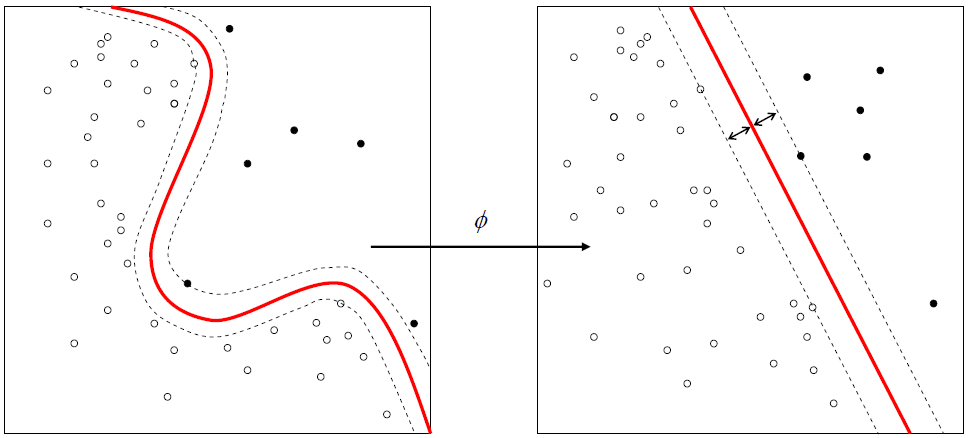
\includegraphics[width=\textwidth]{figures/Kernel_Machine_public.png}
\end{figure}
\end{frame}

% James
\begin{frame}{Support Vector Machines}
It is standard to use the kernel trick to attempt to separate non-linearly separable data without much extra work.\\

We have found that a polynomial of order $p$ works:

\[ k(\mathbf{x}_i,\mathbf{x}_j) = \left(1 + \mathbf{x}_i\cdot\mathbf{x}_j\right)^p. \] 

\begin{figure}[b]
   \centering
   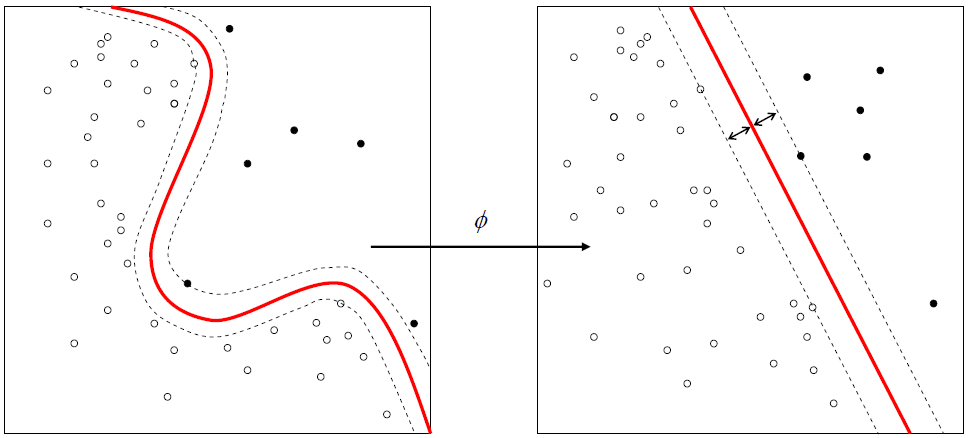
\includegraphics[width=\textwidth]{figures/Kernel_Machine_public.png}
\end{figure}
\end{frame}

% James
\begin{frame}{Support Vector Machines}
   SVMs (as stated) naturally lead to binary classification.  There are a number of ways to extend SVMs to support multiple classes (genres).\\

   ~\\
   One idea is to build $n$ SVM classifiers $f_i$, $i=1,...,n$ that can (hopefully) distinguish between certain subsets of the classes.  By using each of these classifiers, we can hopefully distinguish between multiple classes.\\
   
\end{frame}

% James
\begin{frame}{Support Vector Machines - One vs. All}
   In our context, perhaps the simplest method is compare classical against everything else, electronic against everything else, etc.  The classifier $f_i$ attempts to determine if the test track is of genre $i$ or not.

\begin{table}
   \centering
   \begin{tabular}{|c|cccccc|}
      \hline
      class&$f_1$ & $f_2$ & $f_3$ & $f_4$ & $f_5$ & $f_6$\\\hline
      1 & 1 & 0 & 0 & 0 &0 &0\\\hline
      2 & 0 & 1 & 0 & 0 & 0 & 0\\\hline
      3 & 0 & 0 & 1 & 0 & 0 & 0\\\hline
      4 & 0 & 0 & 0 & 1 & 0 & 0\\\hline
      5 & 0 & 0 & 0 & 0 & 1 & 0\\\hline
      6 & 0 & 0 & 0 & 0 & 0 & 1\\\hline
   \end{tabular}
\end{table}

   Each $f_i$ will give a classification and a score.  We classify the track based on the $f_i$ that gives the optimal score.

\end{frame}

% James
\begin{frame}{Support Vector Machines - One vs. One}
   We can also compare each genre against every other genre.

\begin{table}
   \centering
   \begin{tabular}{|c|ccccccc|}
      \hline
      class&$f_{12}$ & $f_{13}$ & $f_{14}$ & $f_{15}$ & $f_{16}$ & $f_{23}$ & $\cdots$ \\\hline
      1 & 1 & 1 & 1 & 1 & 1 &   & $\cdots$ \\\hline
      2 & 0 &   &   &   &   & 1 & $\cdots$ \\\hline
      3 &   & 0 &   &   &   & 0 & $\cdots$ \\\hline
      4 &   &   & 0 &   &   &   & $\cdots$ \\\hline
      5 &   &   &   & 0 &   &   & $\cdots$ \\\hline
      6 &   &   &   &   & 0 &   & $\cdots$ \\\hline
   \end{tabular}
\end{table}
   
   Each classifier $f_{ij}$ gets a vote for either genre $i$ or genre $j$.  We pick the genre with the most votes.

\end{frame}

% James
\begin{frame}{Support Vector Machines - Error Correcting Output Codes}
   We can also use Error Correcting codes.  The method below is based on a Hamming code.  Each genre is assigned a unique codeword.

\begin{table}
   \centering
   \begin{tabular}{|c|cccccc|}
      \hline
      class&$f_{1}$ & $f_{2}$ & $f_{3}$ & $f_{4}$ & $f_{5}$ & $f_{6}$ \\\hline
      1 & 0 & 0 & 0 & 0 & 0 & 0 \\\hline
      2 & 0 & 1 & 0 & 1 & 0 & 1 \\\hline
      3 & 1 & 0 & 0 & 1 & 1 & 0 \\\hline
      4 & 1 & 1 & 0 & 0 & 1 & 1 \\\hline
      5 & 1 & 1 & 1 & 0 & 0 & 0 \\\hline
      6 & 1 & 0 & 1 & 1 & 0 & 1 \\\hline
   \end{tabular}
\end{table}

   Evaluate each $f_i$ to get a row vector; find the codeword that minimizes the Hamming distance.\\

\end{frame}

% James
\begin{frame}{Support Vector Machines - One vs. All}
   Manually selected features (MFCC, FP, WCH).
   ~\\[-9em]
   \begin{figure}
      \centering
      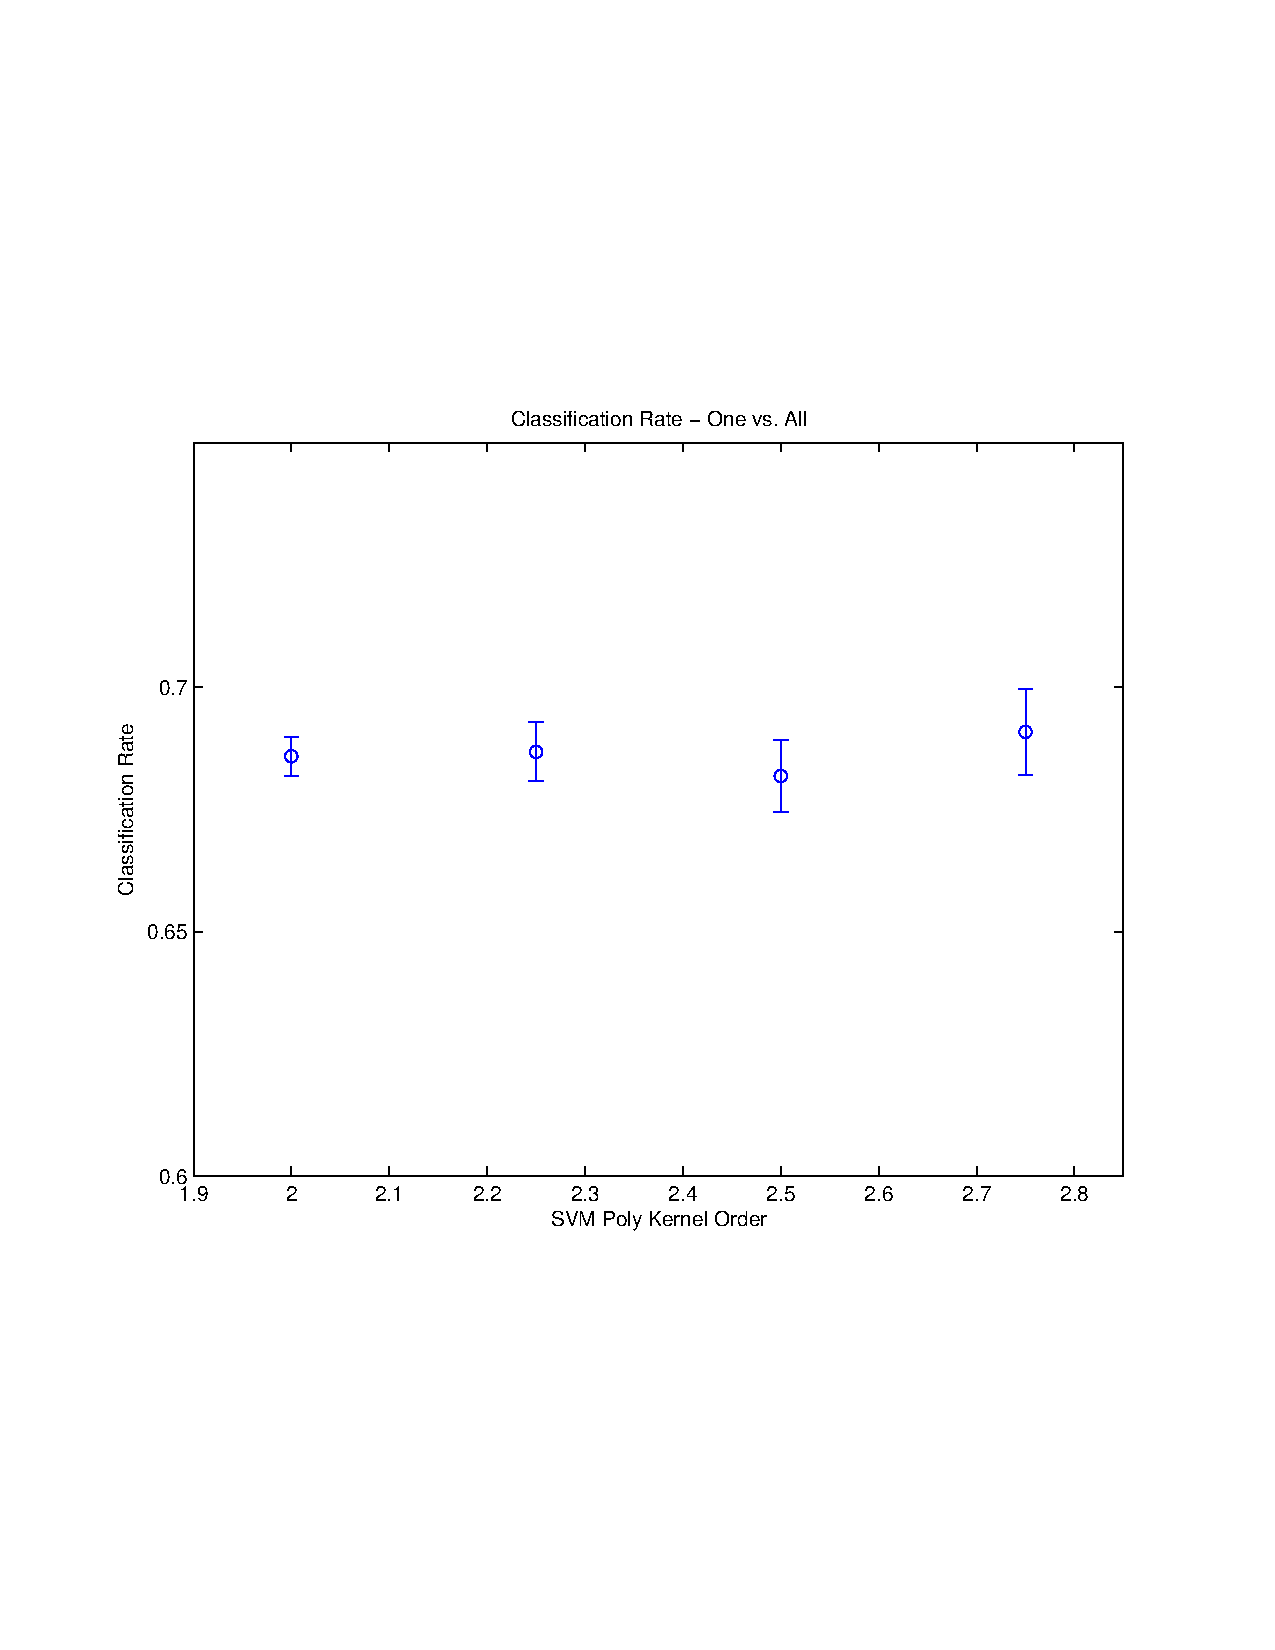
\includegraphics[width=\textwidth]{figures/optimSVMOVAOrder_WCH.pdf}
   \end{figure}
\end{frame}

% James
\begin{frame}{Support Vector Machines - One vs. One}
   Manually selected features (MFCC, FP, WCH).
   ~\\[-9em]
   \begin{figure}
      \centering
      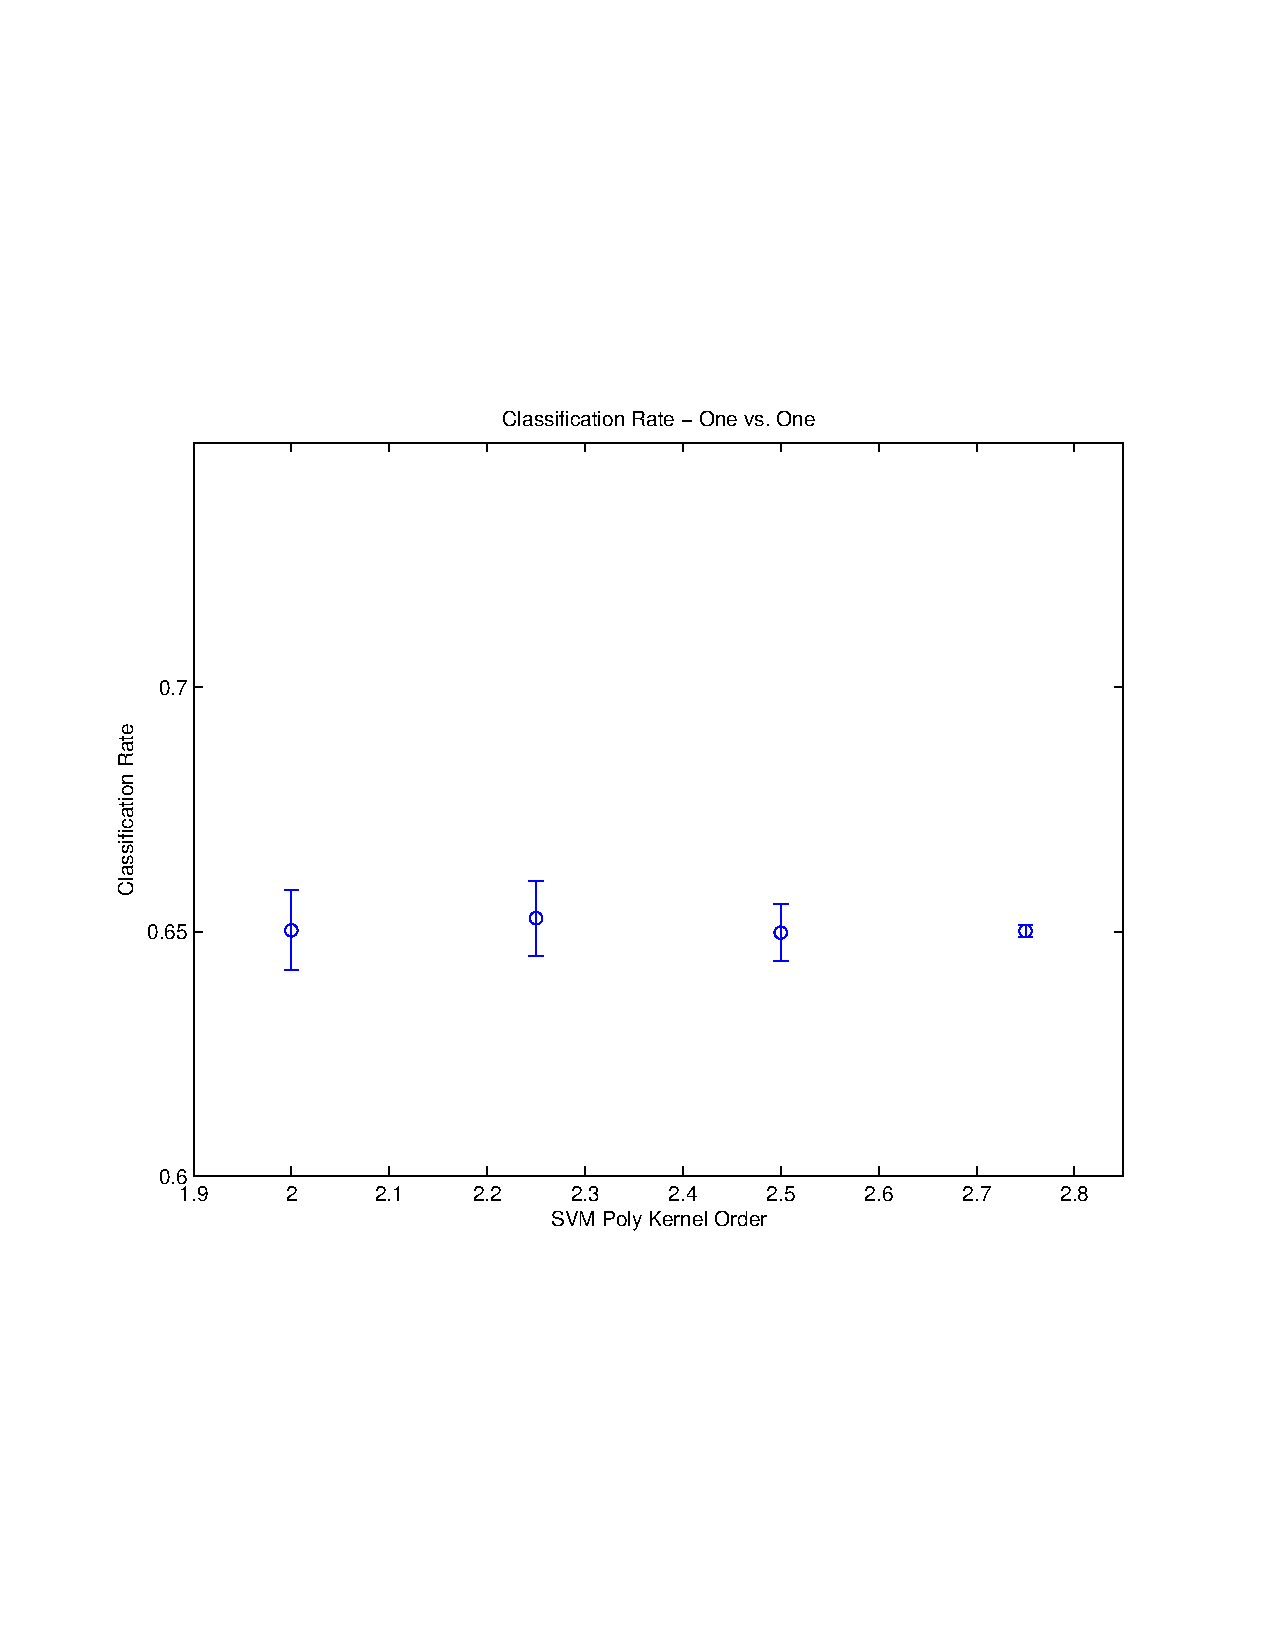
\includegraphics[width=\textwidth]{figures/optimSVMOVOOrder_WCH.pdf}
   \end{figure}
\end{frame}

% James
\begin{frame}{Support Vector Machines - ECOC}
   Manually selected features (MFCC, FP, WCH).  Hamming code.
   ~\\[-9em]
   \begin{figure}
      \centering
      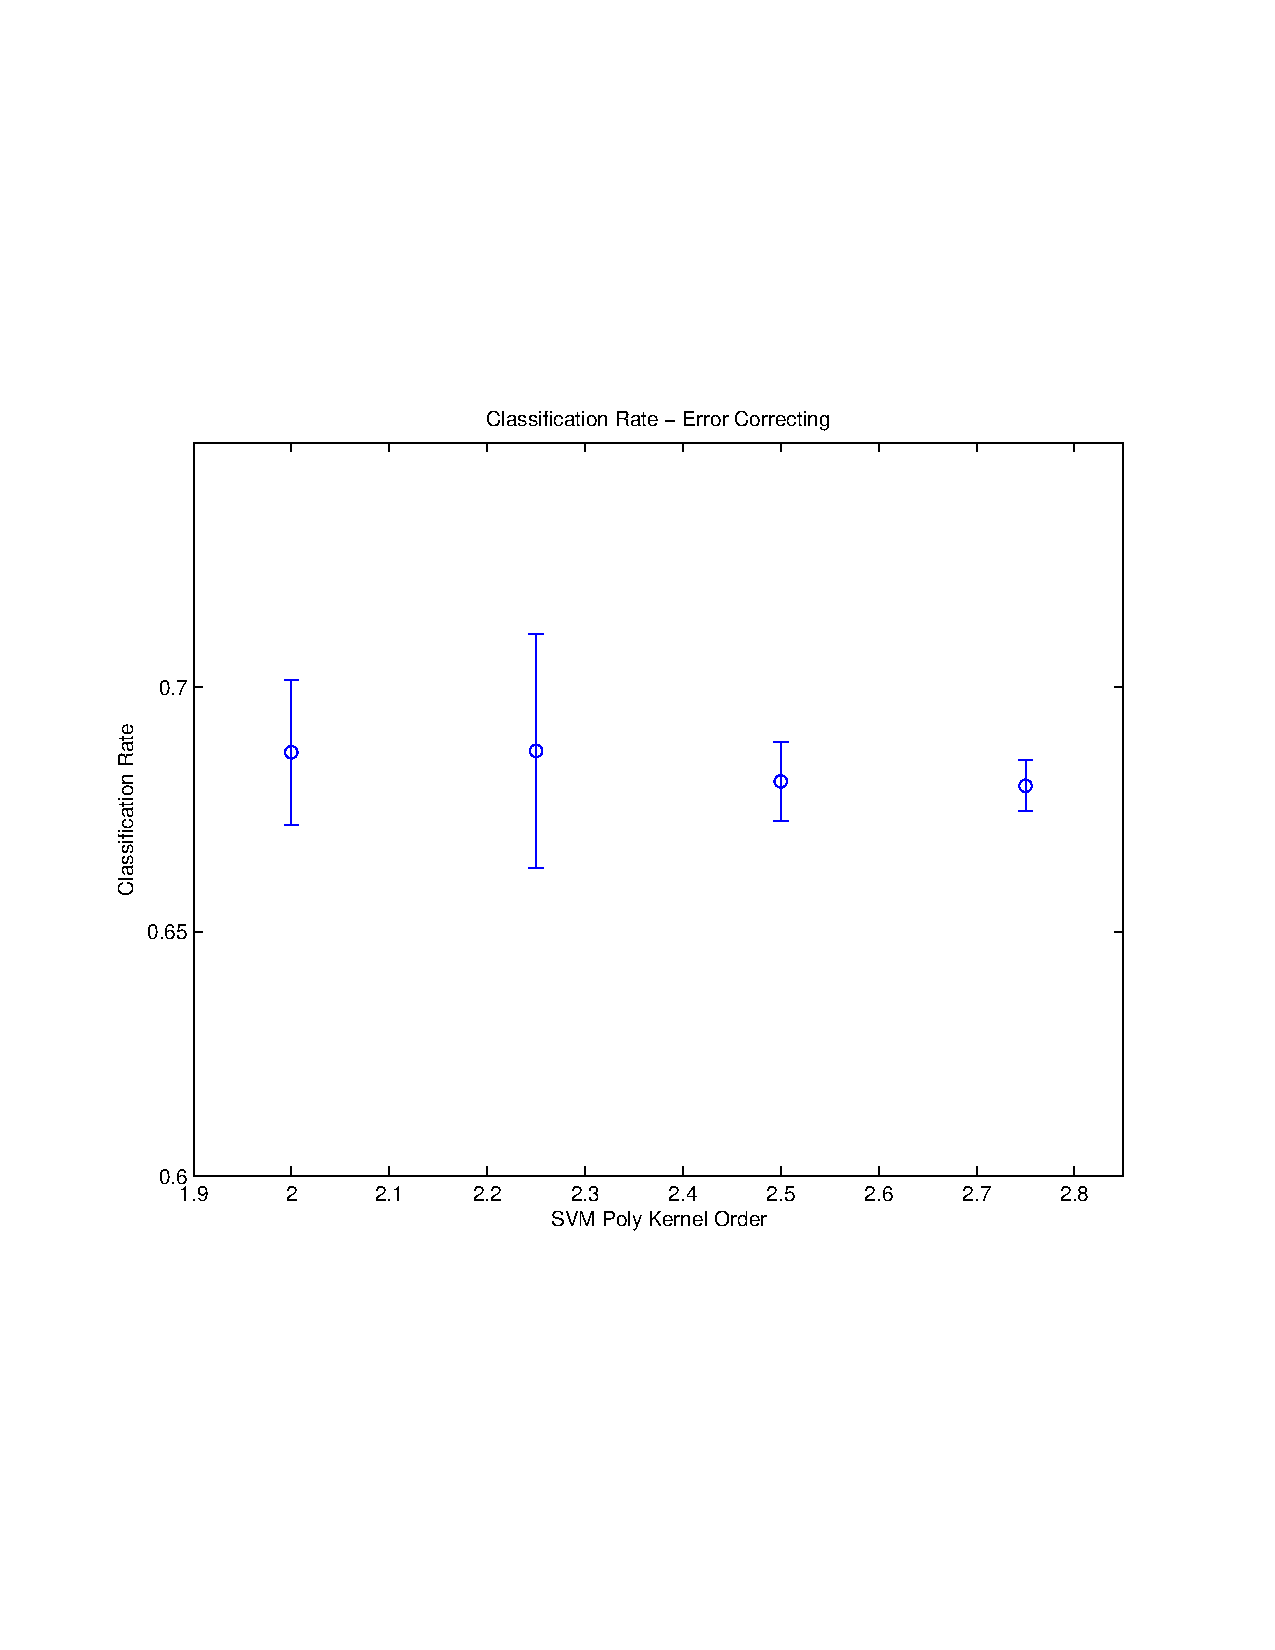
\includegraphics[width=\textwidth]{figures/optimSVMECOCOrder_WCH.pdf}
   \end{figure}
\end{frame}

% James
\begin{frame}[shrink=20]{Support Vector Machines}
   We choose the polynomial order $p=2.25$ with a Hamming-like ECOC.  For this example, we use the manually selected features (MFCC, FP, WCH).  This gives a classification rate of $69.1\%$.

   \begin{table}[h!]
      \centering
         \begin{tabular}{ l||l | l | l | l | l | l | }
         & classical & electronic & jazz\_blues & metal\_punk & rock\_pop & world\\\hline
         classical & 60 &1 &0 &0 &1 &5 \\ \hline 
         electronic & 0 &16 &0 &0 &2 &3 \\ \hline 
         jazz\_blues & 0 &0 &3 &0 &0 &0 \\ \hline 
         metal\_punk & 0 &0 &0 &6 &3 &1 \\ \hline 
         rock\_pop & 1 &3 &1 &2 &14 &3 \\ \hline 
         world & 3 &3 &1 &0 &1 &12 \\ \hline 
         \end{tabular}
      \caption{(Rounded) Average of the Confusion Matrices}
   \end{table}
\end{frame}




\begin{frame}{Graph Results using SVM}
Using SVM one-verse-all method we have the following results: 
\begin{itemize}
\item Unnormalized Spectral Clustering 
\begin{itemize}
\item $\epsilon$-neighborhood: $\epsilon = 0.5$
\begin{figure}[h!]
\centering
  \centering
    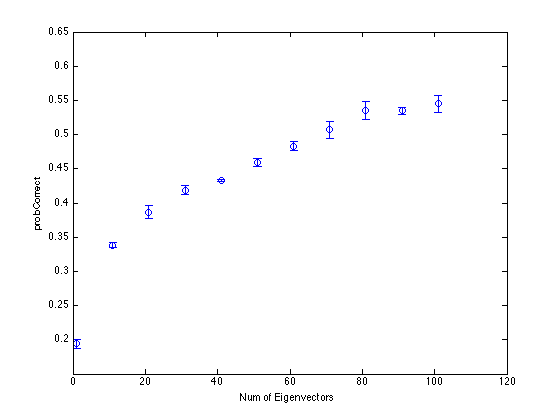
\includegraphics[width=0.7\textwidth]{figures/plotopt1e5.png}
\end{figure}
\end{itemize}
\end{itemize}

\end{frame}

\begin{frame}{Graph Results using SVM}
\begin{itemize}
\item $k$-nearest neighbor graph: $k=2$ 
\begin{figure}[h!]
  \centering
    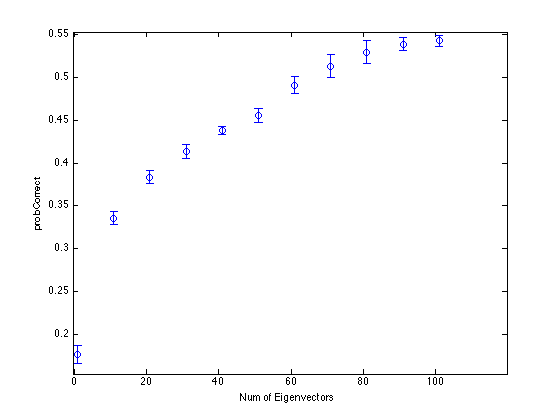
\includegraphics[width=0.7\textwidth]{figures/plotopt2k2.png}
\end{figure}
\end{itemize}
\end{frame}
\begin{frame}{Graph Results using SVM}
\begin{itemize}
\item Connected:  
\begin{figure}[h!]
  \centering
    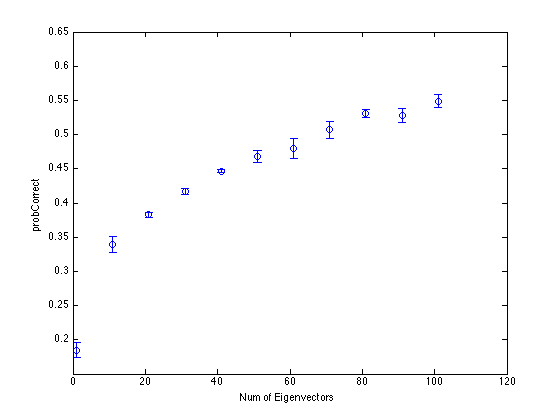
\includegraphics[width=0.7\textwidth]{figures/plotopt3.png}
\end{figure}
\end{itemize}
\end{frame}


\begin{frame}{Graph Results using SVM}
\begin{itemize}
\item Normalized Method 1 Spectral Clustering 
\begin{itemize}
\item $\epsilon$-neighborhood: $\epsilon = 0.5$
\begin{figure}[h!]
\centering
  \centering
    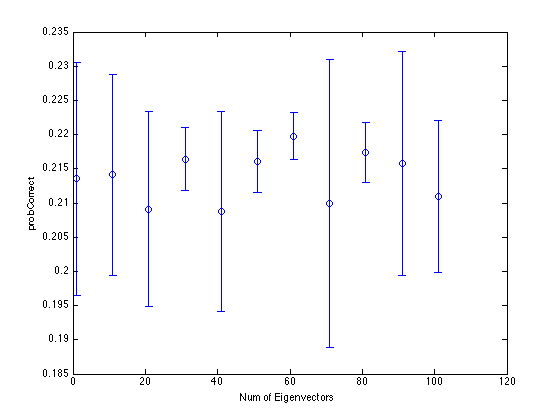
\includegraphics[width=0.7\textwidth]{figures/plotopt1n1.png}
\end{figure}
\end{itemize}
\end{itemize}

\end{frame}

\begin{frame}{Graph Results using SVM}
\begin{itemize}
\item $k$-nearest neighbor graph: $k=2$ 
\begin{figure}[h!]
  \centering
    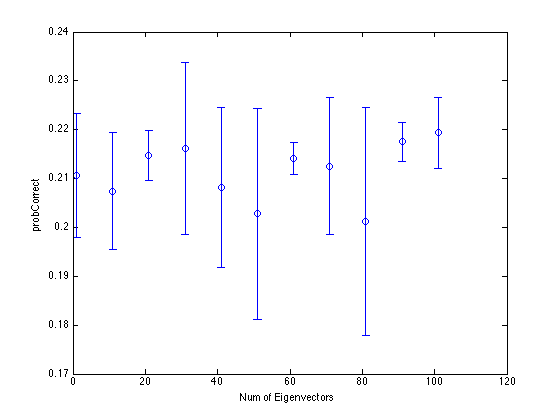
\includegraphics[width=0.7\textwidth]{figures/plotopt2k2n1.png}
\end{figure}
\end{itemize}
\end{frame}
\begin{frame}{Graph Results using SVM}
\begin{itemize}
\item Connected:  
\begin{figure}[h!]
  \centering
    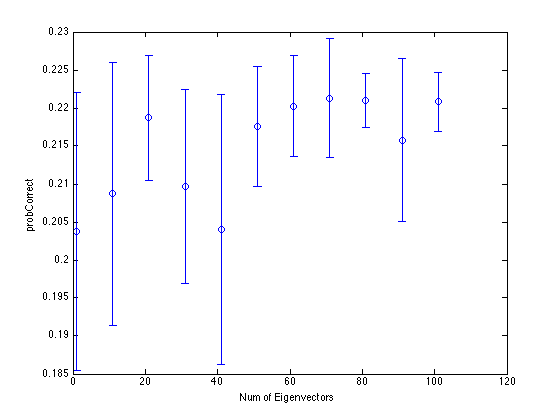
\includegraphics[width=0.7\textwidth]{figures/plotopt3n1.png}
\end{figure}
\end{itemize}
\end{frame}

\begin{frame}{Graph Results using SVM}
\begin{itemize}
\item Normalized Method 2 Spectral Clustering 
\begin{itemize}
\item $\epsilon$-neighborhood: $\epsilon = 0.5$
\begin{figure}[h!]
\centering
  \centering
    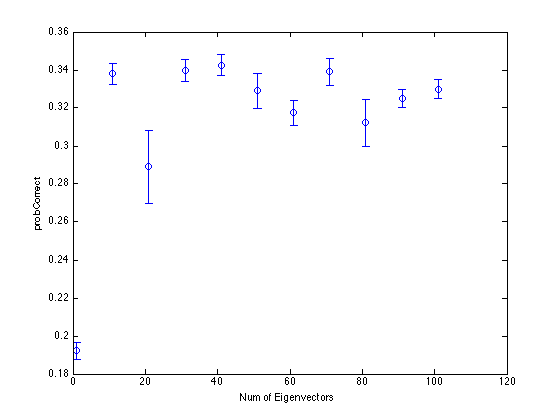
\includegraphics[width=0.7\textwidth]{figures/plotopt1n2.png}
\end{figure}
\end{itemize}
\end{itemize}

\end{frame}

\begin{frame}{Graph Results using SVM}
\begin{itemize}
\item $k$-nearest neighbor graph: $k=2$ 
\begin{figure}[h!]
  \centering
    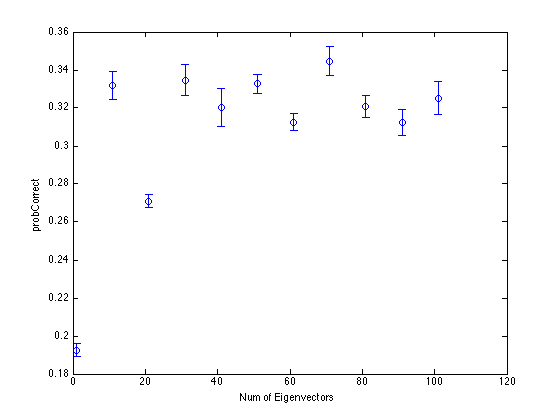
\includegraphics[width=0.7\textwidth]{figures/plotopt2k2n2.png}
\end{figure}
\end{itemize}
\end{frame}
\begin{frame}{Graph Results using SVM}
\begin{itemize}
\item Connected:  
\begin{figure}[h!]
  \centering
    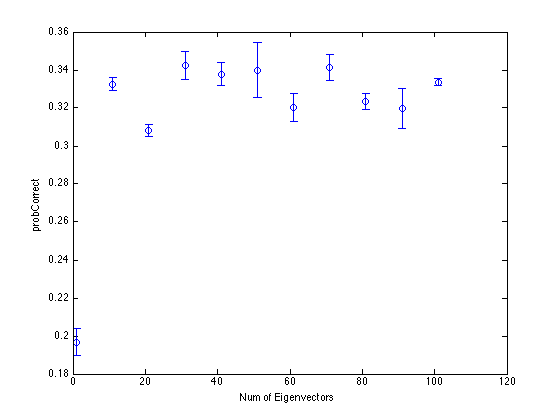
\includegraphics[width=0.7\textwidth]{figures/plotopt3n2.png}
\end{figure}
\end{itemize}
\end{frame}



\section{Discussion}
\begin{frame}{Future Directions}
   \begin{itemize}
      %\item SVM with One vs. All tends to classify world better than the error-correcting codes we've used.  It would be nice to combine One vs. All and an ECOC to get the ``best of both worlds''.\\
      \item The PageRank feature selection lends itself quite naturally to multi-class SVM.  We think it is possible to build a multi-class SVM method tailored to the features selected by the PageRank feature selection.
   \end{itemize}

\end{frame}

\begin{frame}{References}
   % TODO feel free to remove the references
   \setbeamertemplate{description item}[align left] % align left
   \begin{description}                              % align left
      \item[WCH] T. Li, M. Ogihara, Q. Li, \emph{A Comparative Study on Content-Based Music Genre Classification}, SIGIR, (2003).\\
   \end{description}
   ~\\
   Questions?

\end{frame}

\end{document}

% vim: set spell:
% vim: foldmarker=[[[,]]]
